\SourceLeaf{224}%
In der Euklidischen Geometrie gibt es nichts absolut grosses, wohl aber in der Nicht-Euklidischen, diess ist gerade ihr wesentlicher Charakter, und diejenigen, die diess nicht zugeben, setzen eo ipso schon die ganze Euklidische Geometrie; aber, wie gesagt, nach meiner Überzeugung ist diess blosse Selbsttäuschung.

Für den fraglichen Fall ist nun durchaus nichts widersprechendes darin, dass, wenn die Punkte $A$, $B$ und die Richtung $AC$ gegeben sind, während $C$ ohne Beschränkung wachsen kann, dass dann, obgleich so $DBC$ dem $DAC$ immer näher kommt, doch der Unterschied nie unter eine gewisse endliche Differenz heruntergebracht werden könne.

\begin{center}
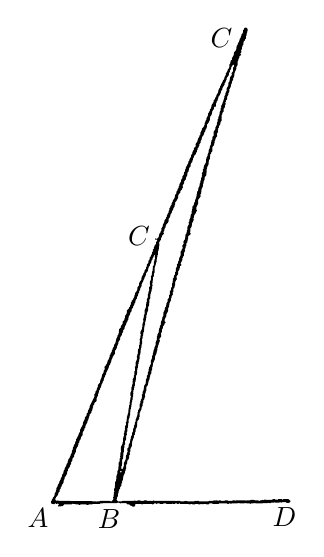
\begin{tikzpicture}[x=0.00551524cm,y=-0.00551524cm]
\fill[even odd rule] (537,24) -- (534,24) -- (532,26) -- (532,28) -- (530,30) -- (530,34) -- (528,38) -- (526,40) -- (526,43) -- (524,46) -- (524,48) -- (522,50) -- (521,55) -- (517,62) -- (517,64) -- (515,66) -- (514,74) -- (512,78) -- (509,81) -- (508,88) -- (506,90) -- (506,92) -- (504,94) -- (505,97) -- (501,101) -- (500,107) -- (498,109) -- (498,115) -- (496,119) -- (494,121) -- (494,123) -- (492,127) -- (490,129) -- (490,133) -- (487,138) -- (486,143) -- (484,145) -- (481,152) -- (479,154) -- (479,156) -- (477,159) -- (477,162) -- (475,164) -- (473,168) -- (472,174) -- (468,180) -- (468,182) -- (465,187) -- (465,189) -- (462,192) -- (462,195) -- (457,203) -- (456,210) -- (453,213) -- (453,216) -- (451,218) -- (451,220) -- (449,222) -- (449,226) -- (445,234) -- (445,237) -- (443,239) -- (443,242) -- (441,244) -- (441,248) -- (438,254) -- (435,257) -- (435,259) -- (431,267) -- (431,271) -- (429,273) -- (429,275) -- (426,280) -- (424,287) -- (420,293) -- (421,297) -- (416,302) -- (417,305) -- (415,307) -- (413,311) -- (413,314) -- (410,318) -- (410,321) -- (406,328) -- (406,330) -- (404,332) -- (403,337) -- (398,346) -- (398,348) -- (396,352) -- (396,355) -- (394,357) -- (393,363) -- (390,367) -- (390,371) -- (388,373) -- (387,375) -- (387,378) -- (383,385) -- (383,388) -- (381,391) -- (381,394) -- (379,396) -- (378,400) -- (376,402) -- (376,406) -- (373,410) -- (372,416) -- (370,420) -- (368,422) -- (367,426) -- (365,429) -- (365,432) -- (362,436) -- (362,438) -- (360,440) -- (360,445) -- (358,447) -- (358,450) -- (354,457) -- (354,460) -- (352,462) -- (352,464) -- (350,466) -- (348,470) -- (348,472) -- (345,478) -- (344,483) -- (341,488) -- (342,491) -- (340,493) -- (339,497) -- (337,499) -- (335,507) -- (331,511) -- (327,510) -- (327,512) -- (328,513) -- (330,512) -- (332,514) -- (332,515) -- (329,519) -- (329,523) -- (326,526) -- (326,528) -- (324,530) -- (324,534) -- (322,536) -- (322,540) -- (320,542) -- (320,546) -- (318,548) -- (317,551) -- (314,555) -- (314,559) -- (312,561) -- (311,567) -- (308,570) -- (308,574) -- (306,577) -- (306,580) -- (303,583) -- (302,588) -- (300,590) -- (300,592) -- (296,599) -- (296,601) -- (295,602) -- (295,606) -- (292,609) -- (292,611) -- (290,613) -- (290,618) -- (286,623) -- (286,628) -- (284,632) -- (282,634) -- (281,636) -- (281,639) -- (279,642) -- (279,644) -- (275,652) -- (273,654) -- (273,656) -- (271,658) -- (271,662) -- (269,665) -- (269,667) -- (267,669) -- (266,672) -- (262,676) -- (262,681) -- (261,682) -- (261,684) -- (258,688) -- (258,693) -- (256,695) -- (256,698) -- (252,702) -- (252,707) -- (248,712) -- (248,715) -- (244,719) -- (243,729) -- (242,730) -- (242,732) -- (240,734) -- (240,737) -- (238,740) -- (235,752) -- (233,754) -- (232,759) -- (229,764) -- (229,766) -- (227,768) -- (227,771) -- (224,776) -- (224,778) -- (222,780) -- (222,784) -- (221,785) -- (220,789) -- (218,791) -- (216,798) -- (213,803) -- (210,806) -- (211,811) -- (208,816) -- (208,819) -- (205,824) -- (203,832) -- (201,835) -- (201,837) -- (200,838) -- (200,842) -- (195,848) -- (195,852) -- (193,855) -- (192,860) -- (189,864) -- (189,867) -- (187,869) -- (187,875) -- (176,897) -- (176,900) -- (172,908) -- (172,911) -- (169,914) -- (169,918) -- (165,923) -- (165,926) -- (161,934) -- (160,940) -- (154,951) -- (154,955) -- (151,960) -- (150,964) -- (148,966) -- (148,968) -- (145,973) -- (145,977) -- (143,979) -- (142,984) -- (140,986) -- (139,990) -- (137,993) -- (137,996) -- (135,1000) -- (135,1004) -- (132,1009) -- (132,1011) -- (129,1017) -- (127,1019) -- (127,1021) -- (125,1025) -- (125,1028) -- (123,1030) -- (122,1034) -- (118,1041) -- (118,1043) -- (116,1046) -- (115,1052) -- (113,1054) -- (112,1059) -- (109,1064) -- (109,1066) -- (106,1071) -- (106,1073) -- (102,1080) -- (102,1082) -- (99,1086) -- (99,1090) -- (98,1091) -- (98,1094) -- (95,1099) -- (95,1102) -- (93,1106) -- (91,1108) -- (91,1110) -- (89,1112) -- (89,1114) -- (87,1116) -- (87,1120) -- (89,1122) -- (92,1122) -- (94,1123) -- (96,1121) -- (98,1121) -- (99,1122) -- (103,1121) -- (105,1123) -- (105,1124) -- (103,1126) -- (103,1128) -- (114,1127) -- (117,1123) -- (134,1123) -- (136,1121) -- (138,1122) -- (143,1122) -- (144,1123) -- (150,1123) -- (151,1124) -- (154,1124) -- (155,1123) -- (168,1123) -- (169,1124) -- (173,1124) -- (174,1123) -- (182,1123) -- (183,1122) -- (199,1122) -- (200,1121) -- (206,1121) -- (207,1120) -- (239,1120) -- (240,1119) -- (243,1119) -- (247,1121) -- (249,1120) -- (260,1120) -- (263,1123) -- (267,1123) -- (270,1126) -- (272,1126) -- (275,1128) -- (279,1128) -- (281,1126) -- (281,1123) -- (282,1122) -- (295,1122) -- (296,1123) -- (298,1123) -- (299,1122) -- (319,1122) -- (320,1123) -- (322,1123) -- (325,1121) -- (329,1121) -- (330,1122) -- (332,1121) -- (337,1121) -- (338,1122) -- (345,1122) -- (346,1121) -- (352,1121) -- (353,1122) -- (366,1122) -- (367,1121) -- (369,1122) -- (372,1122) -- (373,1121) -- (377,1121) -- (378,1122) -- (381,1122) -- (382,1121) -- (384,1121) -- (385,1122) -- (404,1122) -- (405,1123) -- (408,1123) -- (409,1122) -- (412,1122) -- (413,1123) -- (419,1123) -- (420,1122) -- (426,1122) -- (427,1123) -- (444,1122) -- (445,1123) -- (450,1123) -- (452,1121) -- (459,1121) -- (460,1122) -- (473,1122) -- (474,1121) -- (493,1121) -- (494,1122) -- (496,1122) -- (497,1121) -- (500,1121) -- (502,1122) -- (503,1121) -- (516,1121) -- (517,1120) -- (522,1120) -- (523,1121) -- (532,1121) -- (533,1120) -- (537,1120) -- (538,1121) -- (545,1121) -- (547,1122) -- (548,1121) -- (553,1121) -- (554,1120) -- (558,1120) -- (559,1121) -- (574,1121) -- (575,1120) -- (587,1120) -- (588,1119) -- (590,1120) -- (593,1120) -- (594,1119) -- (601,1119) -- (602,1118) -- (604,1119) -- (613,1119) -- (614,1118) -- (619,1119) -- (620,1118) -- (628,1118) -- (629,1119) -- (634,1120) -- (635,1119) -- (637,1119) -- (639,1117) -- (639,1115) -- (634,1111) -- (623,1111) -- (622,1112) -- (620,1112) -- (619,1111) -- (611,1111) -- (609,1113) -- (607,1112) -- (604,1112) -- (603,1111) -- (599,1111) -- (596,1113) -- (582,1113) -- (581,1112) -- (579,1112) -- (576,1114) -- (575,1113) -- (573,1113) -- (572,1114) -- (569,1114) -- (568,1115) -- (566,1115) -- (565,1114) -- (557,1114) -- (556,1113) -- (547,1113) -- (546,1114) -- (538,1114) -- (537,1115) -- (535,1114) -- (514,1114) -- (513,1115) -- (511,1114) -- (506,1114) -- (505,1115) -- (495,1115) -- (494,1114) -- (488,1114) -- (487,1115) -- (479,1115) -- (478,1114) -- (474,1114) -- (473,1115) -- (471,1115) -- (470,1114) -- (467,1114) -- (465,1115) -- (464,1114) -- (462,1114) -- (461,1115) -- (451,1115) -- (450,1116) -- (428,1116) -- (427,1115) -- (424,1115) -- (423,1116) -- (421,1115) -- (419,1115) -- (418,1116) -- (401,1116) -- (400,1115) -- (398,1116) -- (396,1115) -- (394,1116) -- (385,1116) -- (384,1115) -- (377,1115) -- (375,1116) -- (374,1115) -- (325,1115) -- (324,1114) -- (322,1115) -- (308,1115) -- (307,1114) -- (302,1114) -- (301,1115) -- (293,1115) -- (292,1114) -- (287,1114) -- (286,1115) -- (282,1115) -- (280,1114) -- (279,1115) -- (252,1115) -- (251,1116) -- (241,1116) -- (238,1113) -- (239,1107) -- (241,1104) -- (241,1099) -- (243,1095) -- (243,1092) -- (244,1091) -- (244,1089) -- (246,1087) -- (246,1083) -- (249,1080) -- (249,1076) -- (251,1072) -- (251,1069) -- (252,1068) -- (254,1057) -- (257,1051) -- (257,1048) -- (259,1045) -- (259,1042) -- (260,1041) -- (260,1032) -- (262,1030) -- (263,1022) -- (265,1020) -- (267,1016) -- (267,1010) -- (269,1008) -- (268,1004) -- (270,1001) -- (270,995) -- (273,989) -- (274,978) -- (275,977) -- (275,975) -- (278,968) -- (278,964) -- (280,962) -- (280,958) -- (282,955) -- (282,950) -- (285,944) -- (286,931) -- (290,926) -- (290,922) -- (291,921) -- (291,912) -- (293,910) -- (293,908) -- (295,905) -- (296,899) -- (298,896) -- (298,891) -- (300,888) -- (300,883) -- (302,881) -- (302,878) -- (304,875) -- (303,869) -- (305,866) -- (305,864) -- (307,860) -- (307,852) -- (310,848) -- (310,845) -- (311,844) -- (312,838) -- (314,834) -- (314,830) -- (315,829) -- (316,824) -- (318,821) -- (318,815) -- (320,813) -- (320,807) -- (321,806) -- (321,803) -- (322,802) -- (322,798) -- (326,789) -- (327,781) -- (330,775) -- (331,769) -- (332,768) -- (332,762) -- (333,761) -- (333,759) -- (334,758) -- (334,756) -- (335,755) -- (335,753) -- (338,746) -- (337,744) -- (337,741) -- (341,736) -- (341,731) -- (340,729) -- (342,727) -- (343,719) -- (345,716) -- (345,713) -- (348,709) -- (348,707) -- (351,704) -- (351,703) -- (349,701) -- (349,696) -- (353,688) -- (353,684) -- (357,677) -- (357,671) -- (359,667) -- (360,659) -- (363,653) -- (363,649) -- (365,646) -- (365,643) -- (368,639) -- (367,635) -- (369,633) -- (369,626) -- (372,622) -- (372,619) -- (373,618) -- (373,610) -- (375,608) -- (375,606) -- (377,604) -- (376,598) -- (380,592) -- (380,586) -- (383,581) -- (383,579) -- (384,578) -- (384,574) -- (388,571) -- (386,569) -- (386,567) -- (390,559) -- (390,555) -- (391,554) -- (391,552) -- (393,550) -- (393,544) -- (396,538) -- (395,535) -- (397,532) -- (397,529) -- (399,526) -- (399,521) -- (401,519) -- (401,516) -- (402,515) -- (402,512) -- (403,511) -- (403,506) -- (404,504) -- (409,500) -- (409,498) -- (407,496) -- (408,494) -- (408,487) -- (411,483) -- (412,475) -- (416,467) -- (415,463) -- (416,462) -- (417,457) -- (419,453) -- (421,451) -- (421,449) -- (423,447) -- (423,445) -- (422,444) -- (422,438) -- (426,430) -- (426,421) -- (432,413) -- (431,409) -- (433,406) -- (434,396) -- (437,390) -- (437,385) -- (438,384) -- (439,378) -- (441,374) -- (441,369) -- (445,364) -- (446,349) -- (447,348) -- (447,345) -- (450,339) -- (450,333) -- (451,332) -- (451,329) -- (453,327) -- (454,316) -- (456,314) -- (456,312) -- (459,309) -- (459,299) -- (463,294) -- (463,291) -- (464,290) -- (464,285) -- (466,283) -- (466,280) -- (468,276) -- (470,274) -- (469,269) -- (472,264) -- (471,262) -- (472,260) -- (472,256) -- (474,254) -- (474,251) -- (477,247) -- (478,241) -- (480,239) -- (480,226) -- (482,223) -- (482,220) -- (485,217) -- (485,211) -- (488,207) -- (488,202) -- (490,200) -- (489,198) -- (489,195) -- (490,194) -- (490,192) -- (493,189) -- (493,183) -- (496,178) -- (496,175) -- (498,171) -- (498,166) -- (501,161) -- (502,155) -- (504,151) -- (504,148) -- (507,144) -- (507,140) -- (509,137) -- (510,128) -- (514,119) -- (514,115) -- (517,110) -- (517,102) -- (519,99) -- (519,96) -- (521,93) -- (521,90) -- (525,87) -- (525,86) -- (523,84) -- (526,80) -- (525,76) -- (527,73) -- (527,69) -- (528,68) -- (528,66) -- (530,64) -- (531,56) -- (534,53) -- (534,51) -- (536,49) -- (536,44) -- (538,41) -- (538,37) -- (539,36) -- (539,33) -- (540,32) -- (540,27) -- cycle
(246,1047) -- (247,1046) -- (249,1046) -- (250,1048) -- (248,1050) -- (246,1048) -- cycle
(326,548) -- (327,549) -- (327,551) -- (326,552) -- (327,557) -- (325,559) -- (325,563) -- (324,564) -- (324,572) -- (322,574) -- (322,579) -- (321,580) -- (321,585) -- (320,586) -- (319,595) -- (317,597) -- (318,602) -- (317,603) -- (317,606) -- (315,610) -- (315,616) -- (316,618) -- (313,623) -- (313,627) -- (314,629) -- (312,632) -- (311,638) -- (310,639) -- (310,646) -- (308,650) -- (308,656) -- (307,657) -- (307,660) -- (306,661) -- (306,668) -- (303,675) -- (303,684) -- (301,687) -- (301,692) -- (300,693) -- (300,696) -- (299,697) -- (300,699) -- (300,702) -- (298,706) -- (297,718) -- (293,726) -- (293,730) -- (294,731) -- (294,733) -- (293,734) -- (293,739) -- (291,743) -- (292,745) -- (292,748) -- (291,749) -- (291,755) -- (290,756) -- (290,763) -- (288,765) -- (288,768) -- (287,769) -- (287,776) -- (286,777) -- (286,780) -- (285,781) -- (285,784) -- (286,786) -- (285,787) -- (285,789) -- (282,796) -- (282,804) -- (280,807) -- (281,809) -- (281,815) -- (279,817) -- (279,825) -- (278,826) -- (278,830) -- (275,835) -- (276,837) -- (275,839) -- (275,846) -- (274,847) -- (274,850) -- (272,854) -- (272,862) -- (270,866) -- (270,872) -- (271,873) -- (271,876) -- (270,877) -- (270,882) -- (269,883) -- (269,886) -- (268,887) -- (268,894) -- (267,895) -- (267,900) -- (266,901) -- (266,905) -- (265,906) -- (265,912) -- (264,913) -- (264,916) -- (263,917) -- (263,920) -- (262,921) -- (261,932) -- (259,935) -- (260,937) -- (260,940) -- (258,942) -- (257,953) -- (256,954) -- (256,958) -- (255,959) -- (255,963) -- (256,965) -- (254,967) -- (254,970) -- (253,971) -- (253,979) -- (252,980) -- (252,983) -- (248,991) -- (248,999) -- (249,1001) -- (247,1004) -- (247,1011) -- (246,1012) -- (247,1015) -- (245,1018) -- (245,1024) -- (243,1027) -- (243,1036) -- (242,1037) -- (242,1043) -- (240,1047) -- (240,1053) -- (238,1056) -- (237,1069) -- (235,1071) -- (234,1085) -- (232,1088) -- (233,1094) -- (232,1095) -- (232,1100) -- (231,1101) -- (231,1106) -- (230,1107) -- (231,1111) -- (227,1116) -- (224,1116) -- (223,1115) -- (200,1115) -- (199,1116) -- (194,1116) -- (192,1117) -- (191,1116) -- (104,1115) -- (103,1114) -- (99,1115) -- (97,1113) -- (97,1110) -- (99,1106) -- (103,1101) -- (104,1096) -- (107,1093) -- (107,1089) -- (109,1087) -- (109,1084) -- (111,1082) -- (112,1078) -- (114,1076) -- (116,1072) -- (116,1068) -- (118,1064) -- (118,1061) -- (120,1059) -- (124,1052) -- (124,1048) -- (126,1045) -- (126,1042) -- (131,1035) -- (131,1032) -- (133,1030) -- (133,1026) -- (136,1022) -- (136,1018) -- (140,1013) -- (140,1010) -- (144,1002) -- (144,998) -- (145,997) -- (145,995) -- (147,991) -- (149,989) -- (149,987) -- (150,986) -- (150,982) -- (152,980) -- (152,977) -- (155,973) -- (156,968) -- (160,963) -- (160,957) -- (164,950) -- (164,948) -- (166,946) -- (166,942) -- (168,940) -- (168,938) -- (171,934) -- (171,931) -- (173,928) -- (173,925) -- (174,924) -- (174,921) -- (176,919) -- (176,916) -- (180,912) -- (180,909) -- (182,906) -- (183,900) -- (184,899) -- (184,895) -- (187,892) -- (187,889) -- (189,887) -- (190,887) -- (192,884) -- (192,878) -- (195,872) -- (195,869) -- (196,868) -- (198,860) -- (200,858) -- (200,855) -- (202,853) -- (204,845) -- (206,843) -- (206,840) -- (208,838) -- (209,832) -- (211,829) -- (211,827) -- (214,823) -- (214,820) -- (219,810) -- (221,803) -- (224,799) -- (224,797) -- (225,796) -- (227,788) -- (229,785) -- (229,783) -- (234,776) -- (234,769) -- (236,767) -- (239,761) -- (239,759) -- (242,752) -- (242,749) -- (246,743) -- (246,739) -- (248,735) -- (250,733) -- (251,728) -- (253,726) -- (253,722) -- (256,719) -- (257,713) -- (260,708) -- (261,704) -- (263,702) -- (263,700) -- (265,697) -- (266,690) -- (269,685) -- (269,682) -- (273,677) -- (273,673) -- (276,669) -- (276,667) -- (279,662) -- (279,660) -- (281,658) -- (282,652) -- (285,648) -- (285,645) -- (287,642) -- (288,637) -- (290,635) -- (290,631) -- (292,629) -- (293,624) -- (296,619) -- (296,615) -- (297,614) -- (297,612) -- (299,610) -- (300,606) -- (302,603) -- (302,601) -- (305,596) -- (306,590) -- (310,585) -- (310,582) -- (311,581) -- (312,576) -- (315,572) -- (315,570) -- (318,565) -- (318,562) -- (321,558) -- (321,555) -- (323,553) -- (324,549) -- cycle
(508,109) -- (509,110) -- (509,113) -- (507,116) -- (507,124) -- (503,129) -- (504,133) -- (500,138) -- (498,149) -- (496,151) -- (496,157) -- (492,164) -- (492,169) -- (489,175) -- (489,179) -- (487,181) -- (486,189) -- (484,191) -- (484,194) -- (483,195) -- (482,200) -- (479,205) -- (480,208) -- (478,210) -- (478,215) -- (476,218) -- (475,226) -- (473,230) -- (473,234) -- (471,236) -- (471,241) -- (470,242) -- (469,249) -- (467,251) -- (467,253) -- (466,254) -- (466,258) -- (462,264) -- (462,273) -- (459,276) -- (459,282) -- (457,284) -- (455,295) -- (453,297) -- (453,301) -- (450,308) -- (450,312) -- (448,316) -- (448,319) -- (445,325) -- (444,335) -- (440,342) -- (440,344) -- (439,345) -- (439,349) -- (437,351) -- (437,357) -- (435,359) -- (435,361) -- (436,362) -- (435,364) -- (435,368) -- (433,371) -- (433,375) -- (431,378) -- (431,382) -- (430,383) -- (429,390) -- (427,393) -- (426,400) -- (424,402) -- (424,406) -- (423,407) -- (422,415) -- (421,416) -- (421,418) -- (419,422) -- (419,425) -- (417,428) -- (416,433) -- (413,437) -- (413,442) -- (412,443) -- (412,446) -- (411,447) -- (411,453) -- (409,456) -- (408,463) -- (406,466) -- (406,471) -- (404,473) -- (405,477) -- (401,484) -- (401,491) -- (400,492) -- (400,496) -- (399,497) -- (399,499) -- (397,501) -- (396,512) -- (394,514) -- (392,518) -- (393,522) -- (390,526) -- (390,530) -- (391,532) -- (388,536) -- (388,538) -- (386,540) -- (386,548) -- (382,557) -- (382,560) -- (380,564) -- (380,567) -- (377,570) -- (378,573) -- (375,579) -- (375,586) -- (373,588) -- (373,593) -- (371,595) -- (370,600) -- (368,603) -- (368,608) -- (367,609) -- (367,613) -- (366,614) -- (366,621) -- (364,624) -- (364,628) -- (361,632) -- (361,639) -- (359,641) -- (359,647) -- (356,650) -- (356,655) -- (353,660) -- (353,664) -- (352,665) -- (352,667) -- (350,669) -- (349,675) -- (346,681) -- (346,688) -- (344,691) -- (343,697) -- (340,703) -- (340,709) -- (338,712) -- (338,715) -- (336,719) -- (335,727) -- (332,732) -- (332,735) -- (331,736) -- (331,743) -- (328,750) -- (328,756) -- (325,762) -- (325,765) -- (324,766) -- (324,768) -- (323,769) -- (323,773) -- (322,774) -- (322,778) -- (320,781) -- (320,786) -- (317,792) -- (317,800) -- (315,803) -- (315,805) -- (313,807) -- (313,810) -- (312,811) -- (312,816) -- (310,819) -- (310,824) -- (308,827) -- (308,832) -- (306,834) -- (305,845) -- (302,849) -- (300,861) -- (298,864) -- (298,869) -- (296,871) -- (297,873) -- (297,876) -- (296,877) -- (296,880) -- (294,882) -- (294,884) -- (293,885) -- (293,890) -- (291,892) -- (291,901) -- (288,906) -- (288,910) -- (286,912) -- (287,915) -- (286,916) -- (286,918) -- (285,919) -- (285,921) -- (282,928) -- (282,932) -- (280,935) -- (280,939) -- (279,940) -- (278,946) -- (276,950) -- (276,955) -- (274,958) -- (274,962) -- (271,968) -- (271,972) -- (270,973) -- (269,980) -- (266,986) -- (266,991) -- (263,994) -- (263,999) -- (264,1001) -- (262,1005) -- (262,1008) -- (260,1010) -- (259,1020) -- (255,1028) -- (255,1035) -- (254,1036) -- (253,1040) -- (251,1042) -- (250,1042) -- (249,1041) -- (249,1035) -- (250,1034) -- (250,1031) -- (251,1030) -- (251,1020) -- (253,1017) -- (253,1011) -- (254,1010) -- (254,1003) -- (255,1002) -- (255,993) -- (256,992) -- (256,986) -- (258,984) -- (257,979) -- (260,973) -- (260,965) -- (262,962) -- (261,958) -- (263,954) -- (263,947) -- (264,946) -- (265,936) -- (266,935) -- (266,927) -- (268,923) -- (268,919) -- (269,918) -- (269,911) -- (270,910) -- (270,904) -- (271,903) -- (271,899) -- (272,898) -- (272,894) -- (273,893) -- (273,888) -- (274,887) -- (274,883) -- (275,882) -- (275,876) -- (276,875) -- (276,869) -- (277,868) -- (276,865) -- (277,864) -- (277,860) -- (278,859) -- (278,855) -- (279,854) -- (279,850) -- (280,849) -- (280,843) -- (282,839) -- (283,826) -- (285,823) -- (286,809) -- (287,808) -- (288,799) -- (289,798) -- (289,795) -- (290,794) -- (290,789) -- (291,788) -- (291,780) -- (293,776) -- (294,763) -- (295,762) -- (295,759) -- (296,758) -- (295,755) -- (297,753) -- (297,745) -- (296,743) -- (298,740) -- (298,735) -- (299,734) -- (299,730) -- (300,729) -- (300,726) -- (301,725) -- (302,713) -- (303,712) -- (303,709) -- (304,708) -- (304,702) -- (305,701) -- (306,693) -- (307,692) -- (307,686) -- (308,685) -- (308,682) -- (311,675) -- (311,668) -- (313,664) -- (314,650) -- (316,648) -- (316,646) -- (315,645) -- (316,643) -- (316,638) -- (317,637) -- (317,634) -- (319,631) -- (319,627) -- (320,626) -- (320,620) -- (321,619) -- (320,613) -- (321,612) -- (321,607) -- (322,606) -- (322,599) -- (324,597) -- (324,591) -- (326,588) -- (326,577) -- (327,576) -- (327,573) -- (328,572) -- (329,566) -- (330,565) -- (331,554) -- (332,553) -- (332,549) -- (333,548) -- (333,541) -- (335,537) -- (336,527) -- (337,526) -- (336,519) -- (340,513) -- (340,510) -- (342,507) -- (343,503) -- (347,499) -- (346,495) -- (348,492) -- (349,486) -- (351,484) -- (351,481) -- (353,477) -- (356,474) -- (358,470) -- (358,465) -- (361,461) -- (363,453) -- (365,451) -- (366,447) -- (369,442) -- (369,440) -- (372,436) -- (372,433) -- (373,432) -- (373,427) -- (377,422) -- (380,416) -- (380,411) -- (381,410) -- (381,408) -- (385,404) -- (385,401) -- (389,397) -- (389,395) -- (391,392) -- (390,388) -- (394,382) -- (394,378) -- (398,373) -- (398,370) -- (401,364) -- (401,359) -- (404,355) -- (405,349) -- (407,345) -- (409,343) -- (409,339) -- (411,335) -- (413,333) -- (413,330) -- (414,329) -- (414,326) -- (416,323) -- (416,320) -- (421,315) -- (421,313) -- (423,310) -- (423,307) -- (425,305) -- (425,302) -- (427,300) -- (427,298) -- (429,296) -- (429,292) -- (432,289) -- (432,285) -- (434,282) -- (435,276) -- (437,274) -- (440,268) -- (440,266) -- (443,262) -- (443,259) -- (445,257) -- (445,255) -- (446,254) -- (446,248) -- (450,243) -- (453,237) -- (453,232) -- (454,231) -- (454,229) -- (457,225) -- (459,216) -- (462,212) -- (463,207) -- (464,206) -- (467,206) -- (467,199) -- (469,196) -- (469,194) -- (471,192) -- (471,189) -- (472,188) -- (473,183) -- (475,181) -- (478,175) -- (479,170) -- (482,166) -- (482,163) -- (487,155) -- (487,152) -- (489,150) -- (490,146) -- (492,144) -- (492,140) -- (497,133) -- (497,129) -- (499,126) -- (499,123) -- (502,119) -- (502,116) -- (505,111) -- (507,109) -- cycle;
\node[inner sep=0pt] at (480,49) {$C$};
\node[inner sep=0pt] at (290,504) {$C$};
\node[inner sep=0pt] at (57,1155) {$A$};
\node[inner sep=0pt] at (221,1157) {$B$};
\node[inner sep=0pt] at (625,1153) {$D$};
\end{tikzpicture}

\end{center}

\Needspace{9cm}
 Ihr Hineinziehen des Bogens $CD$ macht allerdings den Schluss um vieles captiöser, allein wenn man, was Sie nur angedeutet haben, klar entwickeln will, so müsste es so lauten:

\begin{center}
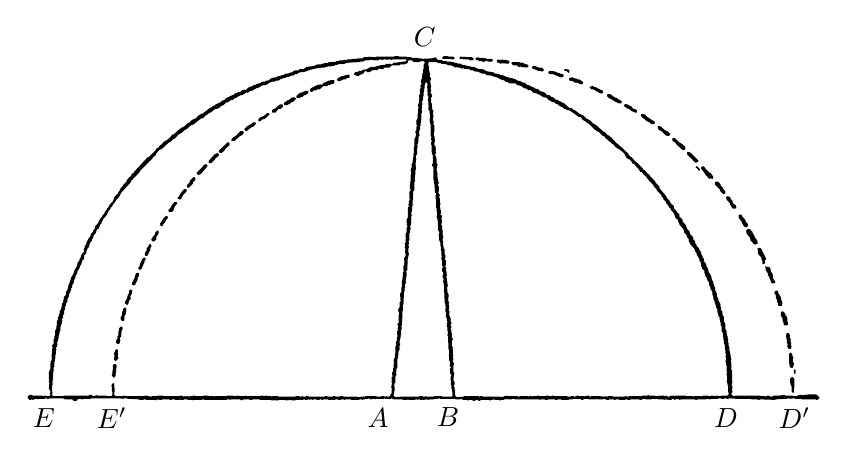
\begin{tikzpicture}[x=0.00688963cm,y=-0.00688963cm]
\fill[even odd rule] (1432,677) -- (1429,680) -- (1429,688) -- (1430,689) -- (1430,692) -- (1432,694) -- (1432,704) -- (1434,706) -- (1435,706) -- (1436,705) -- (1436,697) -- (1437,696) -- (1437,681) -- (1434,677) -- cycle
(1437,663) -- (1436,664) -- (1436,670) -- (1438,671) -- (1439,670) -- (1439,664) -- cycle
(1429,632) -- (1427,634) -- (1427,652) -- (1428,653) -- (1428,658) -- (1431,660) -- (1433,660) -- (1435,658) -- (1435,655) -- (1436,654) -- (1436,652) -- (1434,648) -- (1434,643) -- (1435,642) -- (1435,640) -- (1433,638) -- (1433,635) -- (1430,632) -- cycle
(1423,596) -- (1422,597) -- (1422,600) -- (1421,602) -- (1422,603) -- (1422,607) -- (1424,609) -- (1423,611) -- (1423,614) -- (1425,616) -- (1424,618) -- (1424,621) -- (1426,625) -- (1430,625) -- (1432,621) -- (1431,620) -- (1431,614) -- (1430,613) -- (1430,606) -- (1428,604) -- (1429,600) -- (1426,596) -- cycle
(1414,556) -- (1412,558) -- (1412,564) -- (1415,569) -- (1415,573) -- (1417,577) -- (1417,580) -- (1419,582) -- (1423,582) -- (1425,580) -- (1425,576) -- (1424,575) -- (1424,569) -- (1423,568) -- (1423,566) -- (1420,562) -- (1420,560) -- (1416,556) -- cycle
(1403,518) -- (1400,520) -- (1400,522) -- (1403,527) -- (1403,532) -- (1405,535) -- (1405,538) -- (1407,542) -- (1407,545) -- (1408,546) -- (1413,546) -- (1414,545) -- (1415,540) -- (1412,533) -- (1412,530) -- (1407,522) -- (1407,519) -- (1406,518) -- cycle
(1383,473) -- (1383,475) -- (1384,476) -- (1384,480) -- (1388,486) -- (1388,489) -- (1391,493) -- (1391,495) -- (1392,496) -- (1394,503) -- (1396,505) -- (1398,504) -- (1401,504) -- (1402,502) -- (1398,496) -- (1397,488) -- (1393,481) -- (1393,478) -- (1392,476) -- (1390,474) -- (1385,474) -- cycle
(1370,439) -- (1369,440) -- (1370,450) -- (1376,457) -- (1376,459) -- (1378,463) -- (1378,468) -- (1379,469) -- (1381,469) -- (1383,467) -- (1382,463) -- (1385,460) -- (1385,459) -- (1378,446) -- (1377,442) -- (1374,439) -- cycle
(1352,404) -- (1348,407) -- (1349,413) -- (1355,420) -- (1356,422) -- (1356,425) -- (1360,429) -- (1360,430) -- (1364,433) -- (1368,432) -- (1369,431) -- (1369,427) -- (1367,423) -- (1364,420) -- (1363,416) -- (1360,412) -- (1360,410) -- (1354,404) -- cycle
(1335,378) -- (1334,379) -- (1334,383) -- (1339,390) -- (1343,398) -- (1346,401) -- (1349,401) -- (1351,399) -- (1351,395) -- (1348,392) -- (1346,387) -- (1340,380) -- (1340,379) -- (1339,378) -- cycle
(1313,344) -- (1311,346) -- (1312,350) -- (1318,357) -- (1318,359) -- (1320,361) -- (1322,365) -- (1324,367) -- (1328,367) -- (1330,365) -- (1329,361) -- (1323,356) -- (1323,353) -- (1319,348) -- (1319,346) -- (1318,345) -- cycle
(1292,317) -- (1291,318) -- (1291,323) -- (1300,332) -- (1300,334) -- (1306,340) -- (1308,340) -- (1310,338) -- (1310,335) -- (1305,330) -- (1305,328) -- (1302,325) -- (1300,321) -- (1296,317) -- cycle
(1267,289) -- (1265,291) -- (1265,293) -- (1272,302) -- (1272,303) -- (1280,312) -- (1282,311) -- (1286,312) -- (1287,311) -- (1287,307) -- (1285,305) -- (1285,304) -- (1282,301) -- (1281,301) -- (1272,292) -- (1272,291) -- (1270,289) -- cycle
(1256,289) -- (1255,291) -- (1257,292) -- (1261,297) -- (1262,297) -- (1263,296) -- (1262,293) -- (1258,289) -- cycle
(1239,264) -- (1240,268) -- (1245,273) -- (1246,273) -- (1254,282) -- (1256,282) -- (1260,280) -- (1260,278) -- (1246,264) -- (1241,262) -- cycle
(1212,238) -- (1212,242) -- (1216,244) -- (1219,247) -- (1219,248) -- (1230,258) -- (1234,259) -- (1236,257) -- (1236,253) -- (1229,247) -- (1225,245) -- (1217,237) -- (1213,237) -- cycle
(1185,216) -- (1186,220) -- (1189,223) -- (1191,223) -- (1199,231) -- (1203,233) -- (1206,233) -- (1208,231) -- (1208,229) -- (1204,225) -- (1198,222) -- (1190,215) -- (1186,215) -- cycle
(1154,194) -- (1154,196) -- (1159,201) -- (1160,201) -- (1164,205) -- (1170,208) -- (1172,210) -- (1174,211) -- (1178,211) -- (1180,209) -- (1180,207) -- (1166,198) -- (1162,194) -- (1160,193) -- (1155,193) -- cycle
(1123,176) -- (1123,178) -- (1124,179) -- (1125,179) -- (1128,182) -- (1132,183) -- (1137,187) -- (1144,190) -- (1146,190) -- (1147,189) -- (1147,186) -- (1143,183) -- (1140,183) -- (1136,178) -- (1132,177) -- (1130,175) -- (1128,175) -- (1127,174) -- cycle
(1092,157) -- (1092,160) -- (1095,163) -- (1103,167) -- (1105,169) -- (1114,173) -- (1117,173) -- (1119,171) -- (1119,170) -- (1116,167) -- (1113,166) -- (1110,163) -- (1106,162) -- (1098,156) -- (1093,156) -- cycle
(1060,143) -- (1060,144) -- (1063,147) -- (1067,147) -- (1071,150) -- (1081,155) -- (1085,153) -- (1084,150) -- (1082,148) -- (1080,148) -- (1071,143) -- (1069,143) -- (1066,141) -- (1064,141) -- cycle
(1022,127) -- (1022,130) -- (1023,131) -- (1029,132) -- (1033,135) -- (1037,135) -- (1044,138) -- (1046,138) -- (1048,136) -- (1048,134) -- (1041,129) -- (1037,129) -- (1035,127) -- (1031,127) -- (1029,125) -- (1026,125) -- cycle
(984,115) -- (984,117) -- (986,119) -- (992,119) -- (1006,125) -- (1009,125) -- (1012,123) -- (1012,121) -- (1010,119) -- (1008,119) -- (1007,118) -- (1005,118) -- (1004,117) -- (1002,117) -- (995,114) -- (986,113) -- cycle
(1013,111) -- (1014,113) -- (1017,113) -- (1021,117) -- (1022,117) -- (1022,114) -- (1023,113) -- (1022,111) -- (1019,111) -- (1018,110) -- (1014,110) -- cycle
(954,106) -- (954,108) -- (956,110) -- (958,110) -- (965,113) -- (969,113) -- (970,114) -- (974,114) -- (975,113) -- (975,110) -- (972,107) -- (966,107) -- (959,104) -- (956,104) -- cycle
(916,98) -- (916,100) -- (919,103) -- (926,103) -- (929,106) -- (933,105) -- (934,106) -- (945,107) -- (947,105) -- (947,103) -- (945,101) -- (942,101) -- (936,98) -- (931,98) -- (930,97) -- (917,97) -- cycle
(889,94) -- (889,97) -- (890,98) -- (892,98) -- (896,100) -- (898,99) -- (910,100) -- (912,98) -- (912,96) -- (910,94) -- (907,94) -- (906,93) -- (900,93) -- (899,92) -- (897,93) -- (893,93) -- (891,92) -- cycle
(850,90) -- (850,92) -- (853,94) -- (856,94) -- (857,95) -- (861,95) -- (864,97) -- (865,97) -- (867,95) -- (872,95) -- (873,96) -- (880,96) -- (881,95) -- (881,92) -- (880,91) -- (870,91) -- (869,90) -- (856,89) -- (855,88) -- (851,89) -- cycle
(820,89) -- (821,91) -- (826,91) -- (827,92) -- (837,92) -- (840,94) -- (844,94) -- (846,92) -- (846,90) -- (843,88) -- (822,87) -- cycle
(788,89) -- (789,91) -- (805,91) -- (806,92) -- (809,92) -- (811,90) -- (811,89) -- (809,87) -- (800,87) -- (799,86) -- (791,86) -- cycle
(25,713) -- (25,715) -- (28,719) -- (30,719) -- (31,718) -- (35,719) -- (39,717) -- (42,717) -- (43,718) -- (45,717) -- (56,717) -- (57,716) -- (60,716) -- (61,717) -- (64,717) -- (65,716) -- (90,716) -- (94,718) -- (107,718) -- (110,721) -- (115,721) -- (118,717) -- (123,717) -- (124,718) -- (127,718) -- (128,717) -- (141,717) -- (142,716) -- (196,716) -- (197,717) -- (208,716) -- (209,717) -- (230,718) -- (231,719) -- (238,719) -- (239,718) -- (242,718) -- (243,719) -- (260,719) -- (261,720) -- (265,718) -- (267,719) -- (272,719) -- (273,718) -- (286,718) -- (287,719) -- (290,719) -- (291,718) -- (296,718) -- (297,719) -- (304,719) -- (305,718) -- (307,719) -- (312,719) -- (313,718) -- (319,718) -- (320,719) -- (328,719) -- (329,720) -- (331,719) -- (346,719) -- (347,718) -- (349,718) -- (350,719) -- (391,719) -- (392,718) -- (396,718) -- (398,719) -- (399,718) -- (416,718) -- (419,720) -- (423,718) -- (433,718) -- (434,719) -- (438,719) -- (439,718) -- (452,718) -- (453,719) -- (473,719) -- (474,720) -- (478,720) -- (479,719) -- (481,720) -- (487,720) -- (488,719) -- (499,719) -- (500,720) -- (510,719) -- (511,720) -- (518,720) -- (519,719) -- (532,719) -- (533,718) -- (535,718) -- (536,719) -- (540,719) -- (541,718) -- (543,718) -- (544,719) -- (546,718) -- (548,718) -- (549,719) -- (551,718) -- (557,718) -- (558,719) -- (562,719) -- (563,718) -- (566,718) -- (567,719) -- (569,719) -- (570,718) -- (578,718) -- (579,719) -- (591,719) -- (592,718) -- (596,718) -- (597,719) -- (602,719) -- (603,718) -- (607,718) -- (608,719) -- (610,718) -- (620,718) -- (621,719) -- (635,719) -- (636,718) -- (640,718) -- (642,719) -- (643,718) -- (646,718) -- (647,717) -- (652,717) -- (653,716) -- (654,716) -- (656,718) -- (658,718) -- (659,717) -- (664,717) -- (665,718) -- (667,717) -- (681,717) -- (682,716) -- (684,717) -- (693,717) -- (695,716) -- (699,718) -- (715,718) -- (716,719) -- (724,719) -- (725,718) -- (727,719) -- (738,719) -- (739,718) -- (742,718) -- (743,719) -- (745,718) -- (747,718) -- (748,719) -- (750,719) -- (751,718) -- (753,719) -- (761,718) -- (762,719) -- (764,719) -- (765,718) -- (773,718) -- (774,717) -- (780,717) -- (781,716) -- (783,716) -- (784,717) -- (812,717) -- (813,718) -- (821,718) -- (823,717) -- (827,719) -- (834,719) -- (835,720) -- (837,720) -- (838,719) -- (843,719) -- (846,721) -- (850,720) -- (851,719) -- (854,719) -- (856,721) -- (857,721) -- (860,719) -- (874,719) -- (875,720) -- (877,720) -- (878,719) -- (881,719) -- (882,718) -- (884,718) -- (885,719) -- (893,719) -- (894,720) -- (896,720) -- (897,719) -- (901,719) -- (902,718) -- (906,718) -- (907,717) -- (909,718) -- (916,718) -- (917,717) -- (922,717) -- (923,718) -- (967,718) -- (968,719) -- (970,718) -- (977,718) -- (978,719) -- (982,719) -- (983,718) -- (996,718) -- (997,719) -- (1000,719) -- (1001,718) -- (1007,718) -- (1008,719) -- (1021,719) -- (1022,718) -- (1028,718) -- (1029,717) -- (1043,717) -- (1045,719) -- (1047,719) -- (1051,717) -- (1057,717) -- (1058,718) -- (1072,718) -- (1073,717) -- (1075,718) -- (1085,718) -- (1086,717) -- (1088,717) -- (1091,719) -- (1095,719) -- (1096,718) -- (1104,718) -- (1105,719) -- (1107,719) -- (1108,718) -- (1114,718) -- (1115,719) -- (1125,719) -- (1126,718) -- (1129,718) -- (1130,719) -- (1134,719) -- (1135,718) -- (1151,718) -- (1152,719) -- (1155,719) -- (1158,717) -- (1162,717) -- (1163,718) -- (1174,718) -- (1175,717) -- (1178,717) -- (1180,718) -- (1181,717) -- (1185,717) -- (1186,718) -- (1196,718) -- (1197,719) -- (1199,718) -- (1201,718) -- (1202,719) -- (1204,718) -- (1206,719) -- (1210,719) -- (1212,717) -- (1214,717) -- (1216,719) -- (1221,717) -- (1222,718) -- (1225,718) -- (1226,719) -- (1228,718) -- (1254,718) -- (1255,719) -- (1257,719) -- (1258,718) -- (1274,718) -- (1275,717) -- (1283,718) -- (1284,717) -- (1296,717) -- (1297,716) -- (1302,716) -- (1303,717) -- (1307,717) -- (1308,716) -- (1311,716) -- (1312,717) -- (1315,717) -- (1316,716) -- (1322,716) -- (1324,717) -- (1325,716) -- (1327,716) -- (1328,717) -- (1357,717) -- (1358,718) -- (1369,718) -- (1370,719) -- (1372,719) -- (1373,718) -- (1401,719) -- (1402,718) -- (1423,717) -- (1424,716) -- (1427,716) -- (1428,717) -- (1438,716) -- (1439,717) -- (1449,717) -- (1450,718) -- (1476,718) -- (1477,719) -- (1479,719) -- (1483,716) -- (1483,714) -- (1477,709) -- (1462,709) -- (1461,710) -- (1458,709) -- (1457,710) -- (1454,710) -- (1453,711) -- (1451,710) -- (1445,710) -- (1441,712) -- (1435,712) -- (1434,711) -- (1420,711) -- (1419,710) -- (1416,710) -- (1414,711) -- (1412,710) -- (1411,711) -- (1399,711) -- (1396,713) -- (1393,713) -- (1390,711) -- (1387,711) -- (1384,713) -- (1382,712) -- (1375,712) -- (1374,711) -- (1345,711) -- (1344,712) -- (1342,711) -- (1328,711) -- (1327,712) -- (1324,712) -- (1321,709) -- (1321,707) -- (1323,704) -- (1322,702) -- (1323,695) -- (1321,692) -- (1322,690) -- (1322,687) -- (1323,686) -- (1322,684) -- (1322,665) -- (1321,664) -- (1321,651) -- (1320,650) -- (1320,646) -- (1321,644) -- (1320,643) -- (1319,634) -- (1318,633) -- (1318,630) -- (1317,629) -- (1317,621) -- (1316,620) -- (1316,615) -- (1315,614) -- (1315,606) -- (1314,605) -- (1314,602) -- (1313,601) -- (1313,598) -- (1312,597) -- (1312,592) -- (1310,589) -- (1310,580) -- (1307,574) -- (1307,566) -- (1305,564) -- (1304,556) -- (1302,554) -- (1302,548) -- (1300,546) -- (1301,543) -- (1297,536) -- (1297,533) -- (1294,528) -- (1294,523) -- (1291,517) -- (1291,512) -- (1289,509) -- (1287,501) -- (1285,498) -- (1284,492) -- (1281,486) -- (1279,484) -- (1278,478) -- (1275,473) -- (1275,471) -- (1273,467) -- (1271,465) -- (1270,459) -- (1268,457) -- (1268,454) -- (1266,452) -- (1264,445) -- (1262,443) -- (1261,440) -- (1257,436) -- (1257,434) -- (1254,430) -- (1254,427) -- (1250,423) -- (1251,420) -- (1246,415) -- (1244,411) -- (1244,409) -- (1240,405) -- (1236,396) -- (1231,391) -- (1231,388) -- (1230,386) -- (1225,381) -- (1225,377) -- (1221,374) -- (1221,373) -- (1215,366) -- (1215,363) -- (1214,361) -- (1210,358) -- (1206,351) -- (1202,347) -- (1201,344) -- (1189,330) -- (1188,326) -- (1181,319) -- (1181,317) -- (1171,307) -- (1171,306) -- (1168,303) -- (1167,303) -- (1165,301) -- (1165,300) -- (1161,296) -- (1160,296) -- (1158,294) -- (1158,293) -- (1146,281) -- (1145,281) -- (1137,272) -- (1136,272) -- (1132,268) -- (1130,264) -- (1129,264) -- (1118,253) -- (1117,253) -- (1111,247) -- (1110,247) -- (1099,235) -- (1098,235) -- (1095,232) -- (1092,231) -- (1089,227) -- (1084,224) -- (1072,213) -- (1066,210) -- (1060,204) -- (1054,201) -- (1049,196) -- (1041,192) -- (1032,185) -- (1030,185) -- (1027,182) -- (1022,181) -- (1012,172) -- (1010,172) -- (1008,170) -- (1004,169) -- (1000,166) -- (997,166) -- (993,162) -- (989,161) -- (986,158) -- (982,158) -- (977,153) -- (973,152) -- (972,151) -- (969,151) -- (965,147) -- (958,145) -- (956,143) -- (954,143) -- (949,140) -- (945,139) -- (940,135) -- (938,135) -- (932,132) -- (927,131) -- (922,128) -- (920,128) -- (916,126) -- (912,126) -- (911,125) -- (909,125) -- (908,124) -- (906,124) -- (899,121) -- (896,121) -- (893,119) -- (885,118) -- (883,116) -- (871,114) -- (863,110) -- (855,110) -- (852,108) -- (850,108) -- (848,106) -- (842,106) -- (841,105) -- (838,105) -- (837,104) -- (834,104) -- (833,103) -- (830,103) -- (829,102) -- (825,102) -- (822,100) -- (817,100) -- (816,99) -- (810,98) -- (809,97) -- (806,97) -- (805,96) -- (797,96) -- (796,95) -- (790,95) -- (787,93) -- (780,93) -- (776,88) -- (774,89) -- (771,89) -- (770,90) -- (751,91) -- (750,90) -- (744,90) -- (743,89) -- (732,89) -- (731,88) -- (724,88) -- (723,87) -- (709,87) -- (708,86) -- (701,86) -- (700,87) -- (667,87) -- (666,88) -- (653,87) -- (652,88) -- (644,88) -- (642,90) -- (632,90) -- (631,91) -- (622,91) -- (621,92) -- (614,92) -- (613,93) -- (607,93) -- (606,94) -- (599,94) -- (598,95) -- (594,95) -- (591,97) -- (589,97) -- (588,96) -- (586,97) -- (580,97) -- (576,99) -- (571,99) -- (570,100) -- (567,100) -- (566,101) -- (559,101) -- (553,104) -- (538,106) -- (536,108) -- (532,110) -- (526,110) -- (524,112) -- (518,112) -- (514,114) -- (512,116) -- (509,116) -- (505,118) -- (500,118) -- (496,121) -- (493,121) -- (489,123) -- (486,123) -- (483,125) -- (475,126) -- (468,131) -- (464,131) -- (462,133) -- (457,133) -- (453,136) -- (450,136) -- (449,137) -- (447,137) -- (445,139) -- (442,139) -- (437,142) -- (435,142) -- (430,145) -- (427,148) -- (421,148) -- (416,152) -- (413,152) -- (410,154) -- (408,154) -- (406,156) -- (391,163) -- (387,167) -- (383,168) -- (380,171) -- (371,175) -- (369,177) -- (366,178) -- (363,181) -- (361,181) -- (347,192) -- (345,192) -- (340,195) -- (334,201) -- (332,201) -- (327,204) -- (323,208) -- (319,210) -- (314,215) -- (313,215) -- (311,217) -- (309,217) -- (306,220) -- (305,220) -- (294,230) -- (292,230) -- (285,238) -- (284,238) -- (281,241) -- (278,242) -- (270,250) -- (269,250) -- (265,255) -- (263,255) -- (260,260) -- (248,272) -- (246,272) -- (221,299) -- (221,300) -- (216,304) -- (216,306) -- (214,308) -- (213,308) -- (207,315) -- (207,317) -- (201,323) -- (201,324) -- (195,331) -- (195,333) -- (193,335) -- (191,339) -- (185,345) -- (182,353) -- (174,362) -- (174,364) -- (171,367) -- (171,368) -- (167,373) -- (166,376) -- (163,379) -- (162,382) -- (158,386) -- (155,393) -- (149,400) -- (149,403) -- (146,407) -- (145,410) -- (141,414) -- (141,417) -- (137,422) -- (133,430) -- (133,432) -- (130,436) -- (130,439) -- (128,442) -- (129,446) -- (125,450) -- (123,454) -- (123,456) -- (120,461) -- (120,463) -- (117,466) -- (116,472) -- (110,483) -- (110,485) -- (107,491) -- (105,493) -- (105,496) -- (104,497) -- (103,502) -- (101,505) -- (98,517) -- (96,519) -- (96,521) -- (95,522) -- (96,525) -- (92,529) -- (90,540) -- (88,542) -- (88,547) -- (87,548) -- (87,551) -- (84,556) -- (84,560) -- (83,561) -- (83,563) -- (81,567) -- (81,570) -- (79,574) -- (79,582) -- (78,583) -- (78,588) -- (76,590) -- (76,592) -- (75,593) -- (75,596) -- (76,598) -- (75,599) -- (75,601) -- (74,602) -- (74,606) -- (73,607) -- (73,615) -- (70,619) -- (70,621) -- (71,622) -- (71,624) -- (70,625) -- (70,634) -- (69,635) -- (69,640) -- (70,642) -- (69,643) -- (69,646) -- (67,648) -- (68,650) -- (67,652) -- (67,662) -- (66,663) -- (66,665) -- (64,667) -- (64,681) -- (65,682) -- (64,684) -- (64,686) -- (65,687) -- (64,698) -- (67,703) -- (67,705) -- (66,706) -- (67,710) -- (65,712) -- (59,712) -- (58,711) -- (56,711) -- (55,712) -- (53,712) -- (52,711) -- (34,711) -- (33,710) -- (28,710) -- cycle
(759,134) -- (761,136) -- (761,142) -- (760,143) -- (761,145) -- (761,152) -- (762,153) -- (761,157) -- (763,161) -- (763,163) -- (762,164) -- (762,168) -- (763,169) -- (763,177) -- (764,178) -- (763,180) -- (763,185) -- (765,187) -- (765,192) -- (766,193) -- (766,201) -- (765,202) -- (765,206) -- (766,207) -- (766,210) -- (767,211) -- (767,220) -- (768,221) -- (767,223) -- (767,233) -- (769,235) -- (768,237) -- (768,240) -- (769,241) -- (769,244) -- (768,245) -- (768,249) -- (769,250) -- (769,263) -- (770,264) -- (770,267) -- (771,268) -- (771,275) -- (772,276) -- (771,278) -- (771,284) -- (770,285) -- (770,288) -- (772,290) -- (772,294) -- (773,295) -- (772,297) -- (772,302) -- (773,303) -- (772,305) -- (772,313) -- (773,314) -- (773,320) -- (774,321) -- (774,324) -- (775,325) -- (774,326) -- (775,327) -- (774,328) -- (775,329) -- (775,337) -- (777,339) -- (777,341) -- (776,342) -- (776,349) -- (777,350) -- (777,365) -- (778,366) -- (778,372) -- (779,373) -- (779,379) -- (778,380) -- (778,382) -- (779,383) -- (779,386) -- (780,387) -- (781,407) -- (783,410) -- (783,412) -- (782,413) -- (783,426) -- (785,429) -- (785,435) -- (786,436) -- (786,444) -- (787,445) -- (787,453) -- (788,454) -- (787,456) -- (787,461) -- (788,462) -- (788,471) -- (790,474) -- (790,475) -- (788,477) -- (788,482) -- (790,484) -- (790,489) -- (789,490) -- (789,493) -- (791,496) -- (790,502) -- (791,503) -- (791,506) -- (792,507) -- (792,516) -- (791,518) -- (792,519) -- (793,541) -- (794,542) -- (794,547) -- (795,548) -- (795,550) -- (794,551) -- (794,556) -- (795,557) -- (795,560) -- (796,561) -- (795,563) -- (795,566) -- (797,569) -- (797,574) -- (798,575) -- (798,577) -- (797,578) -- (797,584) -- (798,585) -- (798,592) -- (799,593) -- (798,601) -- (799,602) -- (800,626) -- (801,627) -- (801,636) -- (800,638) -- (801,639) -- (801,646) -- (803,649) -- (803,654) -- (802,656) -- (804,658) -- (804,660) -- (803,661) -- (803,670) -- (805,673) -- (805,675) -- (804,676) -- (804,684) -- (805,685) -- (804,691) -- (805,692) -- (805,698) -- (806,699) -- (806,703) -- (807,704) -- (807,709) -- (808,711) -- (806,713) -- (788,713) -- (787,712) -- (774,712) -- (773,713) -- (760,713) -- (758,712) -- (757,713) -- (753,713) -- (752,712) -- (747,712) -- (746,713) -- (711,713) -- (710,714) -- (706,713) -- (705,714) -- (702,714) -- (699,711) -- (699,709) -- (700,708) -- (700,703) -- (701,702) -- (700,689) -- (702,687) -- (702,677) -- (704,673) -- (703,668) -- (704,667) -- (704,662) -- (706,659) -- (706,643) -- (707,642) -- (708,629) -- (710,626) -- (710,623) -- (709,621) -- (711,618) -- (711,616) -- (710,615) -- (710,610) -- (711,609) -- (711,606) -- (712,605) -- (712,600) -- (713,599) -- (712,597) -- (713,595) -- (712,592) -- (713,591) -- (713,588) -- (714,587) -- (713,583) -- (714,582) -- (714,575) -- (715,574) -- (714,571) -- (715,570) -- (715,556) -- (716,555) -- (716,544) -- (717,543) -- (718,520) -- (719,519) -- (719,513) -- (720,512) -- (720,505) -- (722,503) -- (721,501) -- (721,499) -- (722,498) -- (722,492) -- (723,491) -- (723,485) -- (722,484) -- (722,482) -- (724,480) -- (725,457) -- (726,456) -- (726,453) -- (727,452) -- (727,449) -- (726,448) -- (726,440) -- (727,439) -- (726,433) -- (727,432) -- (727,429) -- (726,427) -- (728,425) -- (728,412) -- (729,411) -- (729,406) -- (730,405) -- (730,402) -- (729,400) -- (731,396) -- (731,387) -- (732,386) -- (731,384) -- (731,382) -- (732,381) -- (732,377) -- (731,375) -- (733,371) -- (733,363) -- (734,362) -- (734,351) -- (735,350) -- (735,335) -- (737,333) -- (737,318) -- (738,317) -- (738,314) -- (737,312) -- (738,311) -- (738,306) -- (739,305) -- (739,296) -- (740,295) -- (740,290) -- (739,289) -- (740,286) -- (739,285) -- (739,283) -- (740,282) -- (740,277) -- (741,276) -- (740,274) -- (740,270) -- (742,266) -- (742,256) -- (743,255) -- (743,251) -- (742,249) -- (744,247) -- (745,234) -- (747,232) -- (746,230) -- (746,224) -- (748,220) -- (747,216) -- (749,213) -- (748,210) -- (749,209) -- (749,205) -- (750,204) -- (750,202) -- (749,201) -- (750,199) -- (750,191) -- (751,190) -- (751,186) -- (750,184) -- (751,183) -- (751,176) -- (752,175) -- (751,170) -- (753,166) -- (753,160) -- (754,159) -- (754,152) -- (755,151) -- (755,146) -- (756,145) -- (756,139) -- (757,138) -- (757,136) -- cycle
(765,96) -- (767,97) -- (778,97) -- (782,99) -- (786,99) -- (787,100) -- (796,101) -- (800,103) -- (805,103) -- (813,107) -- (816,106) -- (817,107) -- (820,107) -- (824,109) -- (828,108) -- (830,110) -- (832,109) -- (834,110) -- (838,110) -- (841,112) -- (845,112) -- (848,114) -- (856,115) -- (858,117) -- (860,117) -- (861,118) -- (867,118) -- (870,121) -- (880,122) -- (881,123) -- (889,125) -- (899,130) -- (902,130) -- (905,133) -- (909,134) -- (912,136) -- (923,136) -- (926,139) -- (934,141) -- (939,145) -- (944,146) -- (947,149) -- (949,148) -- (952,149) -- (957,154) -- (961,154) -- (966,157) -- (968,157) -- (970,159) -- (976,162) -- (979,162) -- (981,163) -- (986,168) -- (988,168) -- (990,170) -- (995,171) -- (998,174) -- (1000,174) -- (1005,178) -- (1010,180) -- (1013,183) -- (1015,183) -- (1018,185) -- (1023,186) -- (1040,198) -- (1043,198) -- (1048,204) -- (1052,206) -- (1055,209) -- (1058,210) -- (1070,222) -- (1071,222) -- (1074,225) -- (1076,225) -- (1084,233) -- (1086,233) -- (1091,239) -- (1092,239) -- (1097,244) -- (1098,244) -- (1102,248) -- (1103,248) -- (1109,255) -- (1114,257) -- (1117,260) -- (1118,260) -- (1124,266) -- (1127,272) -- (1130,275) -- (1133,276) -- (1137,280) -- (1138,283) -- (1139,284) -- (1141,284) -- (1144,287) -- (1144,288) -- (1150,294) -- (1153,299) -- (1155,299) -- (1158,302) -- (1158,303) -- (1165,309) -- (1165,310) -- (1169,314) -- (1169,316) -- (1171,317) -- (1177,323) -- (1178,326) -- (1183,331) -- (1183,333) -- (1192,342) -- (1192,344) -- (1195,347) -- (1196,350) -- (1200,354) -- (1201,357) -- (1204,360) -- (1206,364) -- (1210,368) -- (1210,370) -- (1215,375) -- (1218,384) -- (1223,388) -- (1223,391) -- (1225,394) -- (1225,396) -- (1232,404) -- (1234,408) -- (1234,411) -- (1238,415) -- (1239,419) -- (1242,422) -- (1242,425) -- (1245,432) -- (1253,441) -- (1254,445) -- (1257,449) -- (1257,451) -- (1262,460) -- (1262,463) -- (1264,465) -- (1264,467) -- (1265,468) -- (1265,473) -- (1267,475) -- (1267,477) -- (1271,481) -- (1271,485) -- (1272,486) -- (1273,491) -- (1276,495) -- (1276,498) -- (1278,500) -- (1280,504) -- (1280,508) -- (1282,510) -- (1282,515) -- (1284,517) -- (1286,521) -- (1286,526) -- (1287,527) -- (1288,534) -- (1290,537) -- (1290,540) -- (1291,541) -- (1293,549) -- (1295,552) -- (1295,558) -- (1296,559) -- (1297,564) -- (1299,567) -- (1299,571) -- (1300,572) -- (1300,575) -- (1301,576) -- (1301,581) -- (1303,584) -- (1303,593) -- (1305,595) -- (1305,602) -- (1306,603) -- (1306,608) -- (1307,609) -- (1307,615) -- (1309,618) -- (1309,626) -- (1310,627) -- (1310,634) -- (1311,635) -- (1311,637) -- (1310,638) -- (1310,640) -- (1311,641) -- (1311,646) -- (1310,647) -- (1310,649) -- (1311,650) -- (1311,654) -- (1312,655) -- (1312,666) -- (1313,667) -- (1313,669) -- (1312,670) -- (1312,673) -- (1313,674) -- (1313,683) -- (1312,685) -- (1313,686) -- (1314,692) -- (1315,693) -- (1315,705) -- (1316,706) -- (1316,709) -- (1314,711) -- (1302,711) -- (1301,712) -- (1296,712) -- (1295,711) -- (1293,711) -- (1292,712) -- (1288,712) -- (1287,711) -- (1284,711) -- (1283,712) -- (1278,712) -- (1277,711) -- (1269,711) -- (1268,712) -- (1253,712) -- (1252,713) -- (1250,712) -- (1237,712) -- (1236,711) -- (1218,711) -- (1217,712) -- (1215,712) -- (1214,711) -- (1210,711) -- (1206,713) -- (1203,713) -- (1201,711) -- (1199,712) -- (1197,712) -- (1196,711) -- (1181,712) -- (1180,711) -- (1169,711) -- (1168,710) -- (1166,711) -- (1157,711) -- (1156,712) -- (1133,712) -- (1132,713) -- (1128,713) -- (1127,712) -- (1125,712) -- (1124,713) -- (1103,713) -- (1102,712) -- (1094,712) -- (1093,713) -- (1091,713) -- (1090,712) -- (1088,713) -- (1084,713) -- (1083,712) -- (1081,713) -- (1079,712) -- (1063,712) -- (1062,713) -- (1060,713) -- (1058,711) -- (1052,712) -- (1051,713) -- (1049,712) -- (1040,712) -- (1039,711) -- (1037,711) -- (1033,713) -- (1031,713) -- (1030,712) -- (1026,712) -- (1025,713) -- (1019,713) -- (1018,712) -- (994,712) -- (993,711) -- (991,711) -- (990,712) -- (985,712) -- (984,711) -- (979,711) -- (978,712) -- (967,712) -- (966,711) -- (964,711) -- (963,712) -- (956,712) -- (955,713) -- (953,712) -- (949,712) -- (948,713) -- (946,712) -- (931,712) -- (930,713) -- (928,713) -- (927,712) -- (909,712) -- (907,711) -- (906,712) -- (903,712) -- (900,714) -- (899,713) -- (896,714) -- (895,713) -- (863,713) -- (862,712) -- (859,712) -- (858,713) -- (856,713) -- (855,712) -- (836,712) -- (835,713) -- (833,712) -- (829,712) -- (828,713) -- (815,714) -- (812,711) -- (812,701) -- (811,700) -- (811,696) -- (810,695) -- (810,692) -- (811,691) -- (811,686) -- (809,683) -- (810,672) -- (811,671) -- (809,667) -- (809,655) -- (810,654) -- (809,650) -- (808,649) -- (808,646) -- (809,645) -- (808,639) -- (809,637) -- (808,636) -- (808,626) -- (807,625) -- (808,622) -- (806,619) -- (806,610) -- (808,608) -- (808,607) -- (806,604) -- (806,596) -- (805,595) -- (805,590) -- (804,589) -- (804,587) -- (805,586) -- (805,583) -- (804,582) -- (804,580) -- (805,579) -- (805,576) -- (804,575) -- (804,569) -- (801,562) -- (802,556) -- (800,553) -- (801,551) -- (801,544) -- (800,543) -- (801,539) -- (799,536) -- (800,534) -- (799,532) -- (800,530) -- (800,525) -- (798,521) -- (798,515) -- (797,514) -- (799,507) -- (798,506) -- (798,501) -- (797,500) -- (797,495) -- (796,494) -- (796,492) -- (797,491) -- (796,481) -- (795,480) -- (796,476) -- (794,474) -- (794,472) -- (795,471) -- (795,462) -- (793,460) -- (794,458) -- (794,452) -- (793,451) -- (793,442) -- (791,440) -- (791,436) -- (790,435) -- (790,427) -- (789,426) -- (789,423) -- (790,422) -- (790,416) -- (789,415) -- (789,406) -- (788,405) -- (788,398) -- (787,397) -- (787,394) -- (788,393) -- (787,383) -- (788,382) -- (788,380) -- (785,377) -- (786,375) -- (786,370) -- (785,369) -- (785,365) -- (784,364) -- (784,361) -- (785,360) -- (785,356) -- (784,355) -- (784,348) -- (783,347) -- (783,344) -- (784,342) -- (781,337) -- (782,335) -- (782,326) -- (781,325) -- (781,321) -- (782,320) -- (782,318) -- (781,317) -- (781,313) -- (780,312) -- (780,308) -- (779,307) -- (780,302) -- (779,301) -- (779,297) -- (778,296) -- (778,293) -- (779,292) -- (779,288) -- (780,286) -- (778,283) -- (778,275) -- (777,274) -- (777,270) -- (775,268) -- (775,267) -- (777,265) -- (777,263) -- (776,262) -- (777,257) -- (776,256) -- (776,252) -- (774,250) -- (774,245) -- (775,244) -- (774,233) -- (773,232) -- (773,226) -- (774,225) -- (774,214) -- (772,212) -- (773,207) -- (771,205) -- (771,200) -- (772,199) -- (772,194) -- (771,193) -- (771,191) -- (772,190) -- (772,186) -- (770,184) -- (769,173) -- (768,172) -- (768,162) -- (770,160) -- (770,158) -- (767,154) -- (767,152) -- (768,151) -- (768,148) -- (767,147) -- (768,140) -- (767,139) -- (767,135) -- (766,134) -- (766,132) -- (768,128) -- (765,122) -- (766,118) -- (765,117) -- (765,114) -- (764,113) -- (764,105) -- (763,104) -- (763,98) -- cycle
(756,97) -- (756,99) -- (754,102) -- (754,110) -- (753,111) -- (753,117) -- (752,118) -- (751,127) -- (749,131) -- (749,134) -- (750,135) -- (750,138) -- (748,140) -- (749,144) -- (747,148) -- (747,153) -- (748,155) -- (746,158) -- (746,162) -- (747,163) -- (746,164) -- (745,174) -- (744,175) -- (744,179) -- (745,180) -- (745,182) -- (744,183) -- (744,191) -- (743,192) -- (743,201) -- (741,204) -- (741,212) -- (742,213) -- (742,215) -- (741,216) -- (741,222) -- (739,225) -- (739,227) -- (740,228) -- (740,233) -- (737,239) -- (737,252) -- (736,253) -- (736,266) -- (735,267) -- (736,271) -- (735,272) -- (735,276) -- (734,277) -- (734,282) -- (732,285) -- (732,288) -- (733,290) -- (731,292) -- (731,295) -- (730,296) -- (731,298) -- (731,304) -- (730,305) -- (730,317) -- (729,318) -- (730,320) -- (729,322) -- (729,330) -- (730,331) -- (730,333) -- (728,336) -- (728,348) -- (729,350) -- (727,353) -- (727,358) -- (726,359) -- (727,363) -- (725,365) -- (725,383) -- (723,387) -- (723,393) -- (724,394) -- (723,397) -- (724,398) -- (724,401) -- (723,402) -- (723,410) -- (721,413) -- (721,420) -- (722,421) -- (721,423) -- (721,429) -- (719,431) -- (720,433) -- (720,436) -- (719,438) -- (721,442) -- (720,444) -- (720,449) -- (721,450) -- (721,453) -- (718,459) -- (718,462) -- (719,463) -- (719,465) -- (718,466) -- (719,469) -- (717,473) -- (717,480) -- (718,482) -- (716,484) -- (716,493) -- (715,494) -- (715,498) -- (714,499) -- (714,511) -- (713,512) -- (713,520) -- (711,523) -- (711,529) -- (712,530) -- (711,534) -- (712,535) -- (712,537) -- (710,539) -- (710,548) -- (707,553) -- (708,557) -- (709,558) -- (709,562) -- (708,563) -- (708,574) -- (709,576) -- (706,579) -- (706,581) -- (707,582) -- (707,586) -- (706,587) -- (707,591) -- (705,593) -- (706,603) -- (705,604) -- (705,610) -- (703,613) -- (703,616) -- (704,618) -- (702,621) -- (702,634) -- (701,635) -- (701,641) -- (699,645) -- (699,648) -- (700,649) -- (700,652) -- (699,653) -- (699,660) -- (698,661) -- (698,666) -- (696,669) -- (696,673) -- (697,674) -- (697,676) -- (695,678) -- (695,681) -- (696,682) -- (695,684) -- (696,690) -- (695,691) -- (695,694) -- (694,695) -- (696,699) -- (695,700) -- (695,707) -- (693,709) -- (693,711) -- (691,713) -- (687,713) -- (686,712) -- (684,713) -- (682,713) -- (681,712) -- (676,712) -- (675,713) -- (668,713) -- (667,712) -- (647,712) -- (646,713) -- (639,713) -- (638,714) -- (632,714) -- (631,713) -- (618,713) -- (616,714) -- (615,713) -- (606,713) -- (605,712) -- (600,712) -- (599,713) -- (592,713) -- (591,712) -- (588,712) -- (587,713) -- (577,713) -- (576,712) -- (573,712) -- (572,713) -- (542,713) -- (541,712) -- (538,712) -- (537,713) -- (532,713) -- (531,712) -- (529,713) -- (526,713) -- (525,712) -- (519,712) -- (518,713) -- (487,713) -- (486,712) -- (476,712) -- (474,713) -- (473,712) -- (467,712) -- (466,711) -- (463,711) -- (462,712) -- (459,712) -- (458,711) -- (454,711) -- (453,712) -- (427,712) -- (426,711) -- (424,712) -- (414,712) -- (413,711) -- (410,711) -- (409,712) -- (404,712) -- (403,711) -- (392,711) -- (391,712) -- (370,712) -- (369,713) -- (367,712) -- (358,712) -- (357,711) -- (349,711) -- (348,712) -- (334,712) -- (333,711) -- (329,711) -- (328,712) -- (324,712) -- (323,713) -- (321,713) -- (320,712) -- (318,712) -- (317,713) -- (314,712) -- (312,713) -- (308,711) -- (306,711) -- (305,712) -- (275,712) -- (274,711) -- (264,711) -- (263,712) -- (254,712) -- (253,713) -- (250,713) -- (249,712) -- (246,712) -- (245,711) -- (241,711) -- (240,712) -- (205,712) -- (204,711) -- (201,711) -- (200,712) -- (187,712) -- (184,709) -- (184,706) -- (185,705) -- (185,697) -- (184,695) -- (185,693) -- (184,692) -- (184,689) -- (183,688) -- (181,689) -- (179,693) -- (180,695) -- (180,703) -- (181,704) -- (181,710) -- (179,712) -- (171,712) -- (170,711) -- (154,711) -- (153,710) -- (151,711) -- (148,711) -- (147,712) -- (145,712) -- (143,710) -- (138,710) -- (136,712) -- (134,711) -- (92,711) -- (91,712) -- (72,712) -- (70,710) -- (70,707) -- (71,705) -- (70,704) -- (70,700) -- (69,698) -- (70,697) -- (70,692) -- (71,691) -- (71,688) -- (70,686) -- (71,685) -- (71,682) -- (72,681) -- (71,677) -- (72,676) -- (72,668) -- (73,667) -- (73,659) -- (74,658) -- (74,649) -- (75,648) -- (75,644) -- (76,643) -- (76,636) -- (77,635) -- (77,628) -- (78,627) -- (77,623) -- (79,621) -- (79,618) -- (80,617) -- (79,613) -- (81,610) -- (81,607) -- (82,606) -- (82,601) -- (83,600) -- (83,597) -- (84,596) -- (84,593) -- (85,592) -- (85,585) -- (86,584) -- (86,582) -- (88,578) -- (88,575) -- (89,574) -- (88,570) -- (90,568) -- (90,563) -- (92,561) -- (92,555) -- (94,552) -- (94,547) -- (95,546) -- (96,541) -- (98,538) -- (98,534) -- (101,528) -- (101,524) -- (103,522) -- (103,520) -- (105,517) -- (105,514) -- (107,512) -- (107,508) -- (110,503) -- (111,497) -- (113,495) -- (113,491) -- (116,487) -- (117,481) -- (119,479) -- (121,475) -- (121,473) -- (124,469) -- (125,463) -- (129,459) -- (129,453) -- (133,449) -- (133,445) -- (134,444) -- (134,442) -- (138,437) -- (139,432) -- (141,428) -- (143,426) -- (143,424) -- (146,420) -- (146,417) -- (151,411) -- (152,406) -- (156,403) -- (156,401) -- (158,399) -- (158,397) -- (161,394) -- (161,391) -- (163,389) -- (164,386) -- (171,378) -- (174,371) -- (177,368) -- (178,365) -- (181,362) -- (182,359) -- (185,356) -- (188,351) -- (193,346) -- (197,338) -- (215,318) -- (215,316) -- (217,314) -- (218,314) -- (219,312) -- (230,301) -- (232,297) -- (255,274) -- (255,273) -- (261,268) -- (262,265) -- (267,259) -- (272,257) -- (285,245) -- (288,244) -- (293,239) -- (297,237) -- (302,231) -- (310,226) -- (314,222) -- (317,221) -- (326,213) -- (330,212) -- (344,201) -- (348,200) -- (353,195) -- (357,193) -- (360,190) -- (362,190) -- (368,185) -- (372,183) -- (374,183) -- (378,181) -- (381,178) -- (386,176) -- (391,171) -- (394,171) -- (399,167) -- (402,167) -- (407,163) -- (409,163) -- (411,161) -- (417,158) -- (419,158) -- (425,155) -- (427,153) -- (431,153) -- (435,150) -- (438,150) -- (446,145) -- (449,145) -- (451,143) -- (453,143) -- (456,140) -- (464,139) -- (474,133) -- (479,133) -- (483,131) -- (487,131) -- (491,128) -- (493,128) -- (496,126) -- (500,126) -- (502,124) -- (506,124) -- (510,122) -- (514,122) -- (516,120) -- (518,119) -- (521,119) -- (525,116) -- (535,115) -- (536,114) -- (539,114) -- (541,112) -- (544,112) -- (545,111) -- (548,111) -- (549,110) -- (552,110) -- (553,109) -- (556,109) -- (557,108) -- (564,108) -- (565,107) -- (572,107) -- (573,106) -- (576,106) -- (577,105) -- (584,105) -- (585,104) -- (589,104) -- (592,102) -- (595,102) -- (596,101) -- (609,100) -- (610,99) -- (614,99) -- (615,98) -- (636,97) -- (637,96) -- (642,96) -- (646,94) -- (653,94) -- (654,93) -- (662,93) -- (663,94) -- (667,93) -- (669,94) -- (673,92) -- (676,92) -- (677,93) -- (679,93) -- (680,92) -- (686,92) -- (687,93) -- (689,92) -- (693,92) -- (694,93) -- (696,93) -- (697,92) -- (722,92) -- (723,94) -- (720,96) -- (714,96) -- (713,97) -- (708,97) -- (707,98) -- (699,98) -- (696,101) -- (694,101) -- (693,100) -- (691,100) -- (690,101) -- (686,100) -- (683,102) -- (673,103) -- (672,104) -- (669,104) -- (665,106) -- (657,106) -- (647,111) -- (643,111) -- (640,113) -- (636,113) -- (633,115) -- (629,115) -- (626,118) -- (626,119) -- (628,121) -- (634,123) -- (636,121) -- (640,119) -- (642,119) -- (647,113) -- (652,116) -- (653,115) -- (656,115) -- (659,112) -- (663,112) -- (664,111) -- (668,112) -- (672,109) -- (679,110) -- (683,107) -- (691,107) -- (696,103) -- (709,103) -- (712,101) -- (720,101) -- (721,100) -- (723,100) -- (725,98) -- (725,95) -- (726,94) -- (733,94) -- (736,97) -- (746,97) -- (750,95) -- (754,95) -- cycle
(187,653) -- (184,653) -- (182,655) -- (182,664) -- (181,665) -- (181,671) -- (180,672) -- (180,674) -- (183,678) -- (184,678) -- (187,675) -- (187,670) -- (188,669) -- (188,661) -- (189,660) -- (189,656) -- cycle
(190,626) -- (188,626) -- (186,628) -- (186,630) -- (184,633) -- (184,635) -- (185,636) -- (184,645) -- (186,647) -- (188,647) -- (192,643) -- (192,641) -- (191,640) -- (191,627) -- cycle
(198,584) -- (196,584) -- (193,588) -- (193,592) -- (192,593) -- (192,600) -- (190,603) -- (190,607) -- (188,609) -- (188,614) -- (190,616) -- (192,616) -- (195,614) -- (195,611) -- (196,610) -- (195,608) -- (195,605) -- (197,602) -- (198,592) -- (200,588) -- (200,586) -- cycle
(204,549) -- (203,549) -- (201,552) -- (201,554) -- (199,557) -- (199,562) -- (196,568) -- (196,570) -- (199,574) -- (201,574) -- (203,572) -- (203,566) -- (206,560) -- (207,551) -- cycle
(216,516) -- (214,516) -- (212,518) -- (212,521) -- (209,527) -- (208,532) -- (204,539) -- (204,541) -- (208,544) -- (210,543) -- (212,536) -- (215,533) -- (214,528) -- (217,523) -- (217,520) -- (218,519) -- (218,518) -- cycle
(229,485) -- (226,485) -- (224,487) -- (222,494) -- (217,504) -- (217,506) -- (219,508) -- (221,508) -- (224,506) -- (224,504) -- (227,499) -- (228,493) -- (230,491) -- (230,486) -- cycle
(241,457) -- (239,457) -- (235,461) -- (235,463) -- (232,468) -- (231,473) -- (229,475) -- (229,478) -- (230,479) -- (233,479) -- (236,476) -- (236,473) -- (238,471) -- (238,469) -- (240,466) -- (240,464) -- (242,460) -- (242,458) -- cycle
(251,432) -- (250,432) -- (248,434) -- (247,437) -- (244,440) -- (244,444) -- (241,448) -- (241,453) -- (242,454) -- (245,454) -- (246,453) -- (246,451) -- (248,449) -- (248,447) -- (251,444) -- (251,439) -- (253,437) -- (253,434) -- cycle
(264,407) -- (260,411) -- (259,415) -- (256,418) -- (253,423) -- (253,425) -- (255,427) -- (258,427) -- (262,423) -- (262,418) -- (264,416) -- (266,412) -- (266,409) -- cycle
(281,380) -- (280,380) -- (274,386) -- (274,387) -- (269,394) -- (269,397) -- (271,399) -- (273,399) -- (274,398) -- (275,395) -- (278,392) -- (279,389) -- (283,384) -- (283,382) -- cycle
(299,355) -- (295,355) -- (290,361) -- (289,364) -- (284,370) -- (284,371) -- (286,373) -- (290,373) -- (293,371) -- (296,362) -- (300,358) -- (300,356) -- cycle
(316,331) -- (313,331) -- (309,335) -- (309,336) -- (305,341) -- (304,344) -- (301,347) -- (302,349) -- (306,350) -- (308,348) -- (311,342) -- (317,336) -- (318,333) -- cycle
(332,309) -- (330,309) -- (324,315) -- (323,319) -- (318,324) -- (318,327) -- (319,328) -- (322,328) -- (329,321) -- (329,319) -- (334,314) -- (334,311) -- cycle
(354,285) -- (350,286) -- (348,288) -- (348,289) -- (336,301) -- (336,302) -- (339,305) -- (344,303) -- (356,289) -- (356,287) -- cycle
(375,264) -- (369,267) -- (359,278) -- (358,281) -- (360,283) -- (363,283) -- (370,276) -- (370,275) -- (377,269) -- (377,267) -- cycle
(395,245) -- (393,245) -- (377,260) -- (377,262) -- (379,264) -- (382,264) -- (384,263) -- (388,259) -- (388,258) -- (394,252) -- (396,251) -- (397,247) -- cycle
(423,226) -- (421,224) -- (417,224) -- (408,233) -- (403,236) -- (400,239) -- (400,241) -- (401,242) -- (406,242) -- (415,234) -- (420,231) -- (422,229) -- cycle
(445,209) -- (444,208) -- (440,208) -- (438,210) -- (428,216) -- (424,220) -- (424,221) -- (427,224) -- (428,224) -- (437,217) -- (440,216) -- (445,211) -- cycle
(470,192) -- (469,191) -- (466,191) -- (460,196) -- (453,199) -- (450,202) -- (450,205) -- (451,206) -- (453,206) -- (458,202) -- (461,202) -- (470,194) -- cycle
(495,176) -- (494,175) -- (490,175) -- (488,176) -- (480,183) -- (478,183) -- (475,186) -- (475,189) -- (476,190) -- (481,190) -- (487,183) -- (491,183) -- (495,179) -- cycle
(519,164) -- (517,162) -- (513,162) -- (509,164) -- (506,167) -- (504,167) -- (499,171) -- (498,171) -- (497,172) -- (497,175) -- (498,176) -- (503,176) -- (504,175) -- (506,175) -- (512,170) -- (514,170) -- (519,165) -- cycle
(542,151) -- (541,150) -- (536,150) -- (530,153) -- (527,153) -- (520,159) -- (520,162) -- (521,163) -- (526,163) -- (529,161) -- (531,161) -- (534,158) -- (536,158) -- (542,154) -- cycle
(590,131) -- (589,130) -- (583,130) -- (582,131) -- (579,131) -- (574,134) -- (570,135) -- (567,139) -- (565,138) -- (559,139) -- (547,145) -- (545,147) -- (545,150) -- (547,152) -- (549,152) -- (552,149) -- (556,149) -- (558,147) -- (563,147) -- (569,141) -- (576,141) -- (579,139) -- (582,139) -- (585,137) -- (588,137) -- (590,135) -- cycle
(618,122) -- (616,120) -- (614,120) -- (613,121) -- (610,121) -- (606,123) -- (603,123) -- (597,126) -- (595,128) -- (595,130) -- (597,132) -- (600,132) -- (606,129) -- (610,129) -- (613,126) -- (617,126) -- (618,125) -- cycle;
\node[inner sep=0pt] at (756,51) {$C$};
\node[inner sep=0pt] at (180,752) {$E'$};
\node[inner sep=0pt] at (670,752) {$A$};
\node[inner sep=0pt] at (799,751) {$B$};
\node[inner sep=0pt] at (1311,752) {$D$};
\node[inner sep=0pt] at (1437,752) {$D'$};
\node[inner sep=0pt] at (55,753) {$E$};
\end{tikzpicture}

\end{center}

Es ist

\[
CAB:CBD=\frac{CD}{ECD}:\frac{CD'}{E'CD'}
\]

\noindent und indem $AC$ ins Unendliche wächst, kommen $CD$ und $CD'$ einerseits und $ECD$, $E'CD'$ andererseits der Wahrheit immer näher.

Beides ist in der Nicht-Euklidischen Geometrie nicht wahr, wenn man darunter versteht, dass ihre geometrischen Verhältnisse der Gleichheit so nahe kommen wie man will. In der That ist in der Nicht-Euklidischen Geometrie
